\section{Architectural Design}
\subsection{Overview}
The figure shown below represents an high-level description of the components which make up the System.
The architectural design of the System is divided between eMSP and CPMS. \\
The former describes the part of the System dedicated to offer a Web App for 
EV Drivers to plan their charges, book a charge and manage the charges. \\
The latter whereas describes the second part of the System used by the CPOs 
to manage the reservations, the CP, the energy mix and the contracts with the DSOs.
Both the two parts consists of a three tier architecture to ensure high maintainability, scalability and security. 


\subsection{Component view}
This figures describes an high-level view of the components of the eMSP and CPMS that will be described in terms of their subcomponents in the next subsections.

\begin{figure}[H]
    \centering
    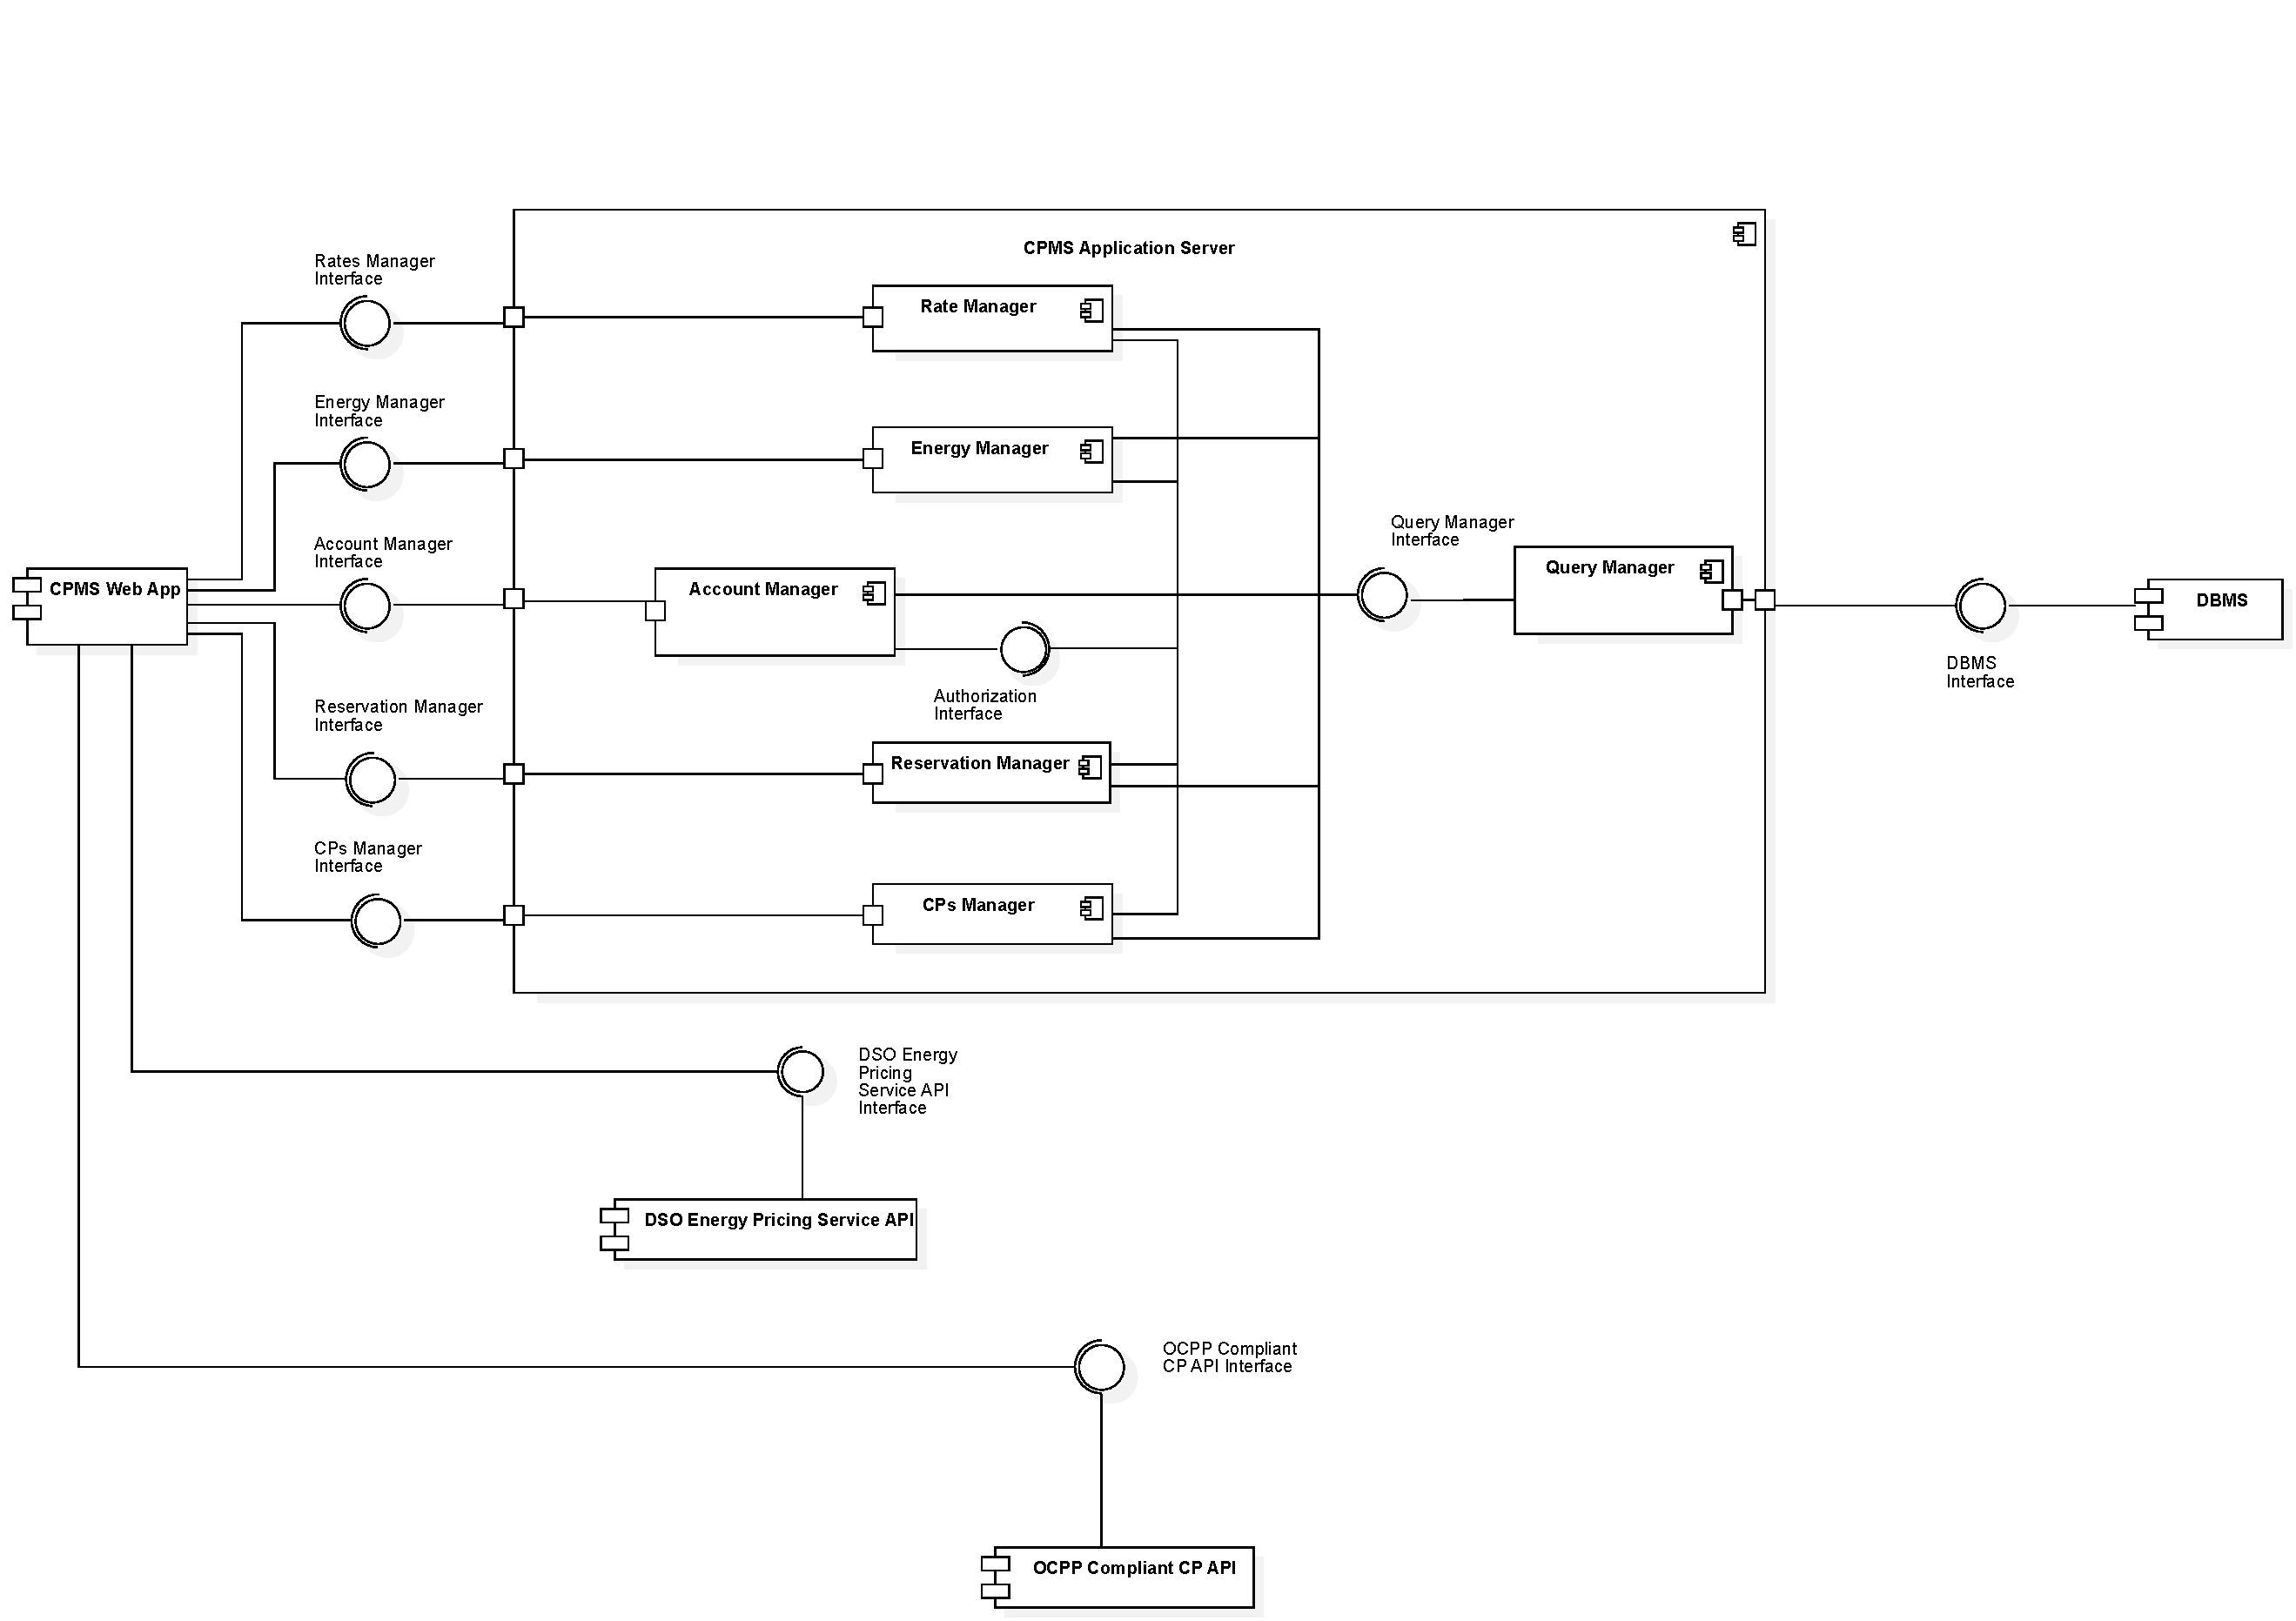
\includegraphics[scale=0.38]{src/ComponentDiagram/CPOdiagram.pdf}
    \caption{Charging Point Operator}
\end{figure} \vspace{1cm}

\subsubsection{CPMS Web App}
It represents the application dedicated to the different CPOs using the system. This component contains the logic to receive HTTPS requests from the users' browser,
forward them to the CPMS Application Server, and generate dynamic pages based on the response from the CPMS Application Server. (For the eMSP) It can be wrapped into a PWA to generate a downloadable application that 
the mobile operating system renders as a native application.

\subsubsection{CPMS Application Server}
The CPMS Application Server is responsible for the business logic to provide the functionality to the application for the CPOs and to coordinate.
the information flow between application layer and data layer.
It is composed of several components, each of them used for a specific functionality:\\
\begin{itemize}
    \item \textbf{Account Manager} \\ This component handles all the account operations related to the CPO and offers an interface to authenticate the requests in the CPMS application server.
    It offer functionality to create new account, logging in, setting preferences and verify the authentication of the user at any time. 
    To create a new account interacts with the external SMS API to make the user receive a code to verify the identity. 
\end{itemize}


\subsection{Deployment view}
Infrastructure: deployment diagram(s) including non-logical elements (e.g., load balancer, firewall)
\subsection{Runtime view}
You can use sequence diagrams to describe the way components interact to accomplish specific tasks typically related to your use cases. Dynamics of the interactions: sequence
diagrams (realization of use cases)
\subsection{Component interfaces}
Details for each interface (name, signature, returned objects)
\subsection{Architectural Styles and patterns}
Please explain which styles/patterns you used, why, and how
\subsection{Other design decisions}